% !TeX spellcheck = en_GB
\chapter{Methods}

\section{Microscope setup}

\begin{figure}[bh]
	\centering
	\includegraphics[width=\linewidth]{microscope layout.pdf}
	\caption{
		Schematic overview of the Tegenfeldt microscope. The sample is located in a microscope housing on the bottom right (outside this figure). FC1 and FC2 are swappable filter cubes. Half-wave and quarter-wave plates are denoted $ \lambda/2 $ and $ \lambda/4 $, respectively. Dashed lines represent the light path, except those that go to the TCSPC (those are digital connections). The waveplates in the pSTED module were not in the original setup, and were added as part of this project. See text for more details.
	}
	\label{fig:layout}
\end{figure}

The Tegenfeldt microscope is a confocal fluorescence microscope constructed by Abberior Instruments GmbH (Germany). It features two excitation lasers (at 561~nm and 640~nm) and one depletion laser at 775~nm for two-channel confocal or STED microscopy. It also contains a time-correlated single photon counter (TCSPC) for fluorescence lifetime imaging microscopy (FLIM) and a highly sensitive photomultiplier tube (PMT). Refer to \autoref{fig:layout} for the layout of these optical elements. Samples are located inside an inverted Nikon microscope body (Ti-E, not shown in the figure) equipped with a piezo stage (M-687 PILine XY-stage system and P-736 PInano (Physik Instrumente) Z Microscope Scanner), a 60x, 1.4~NA oil immersion objective (Nikon Plan Apo) and a QUADScan beam scanner (Cambridge Technology).


In this section, I will address all laser lines as well as the detection module in detail, with a focus on characterising the light polarisation at different points in the microscope.

\paragraph{The laser modules.} This fast-switching 561~nm laser is initially horizontally polarised, but the polarisation can be tuned by three waveplates in its path. The last one, a quarter-wave plate, is fixed in its rotation angle. In the standard mode of operation, excitation laser light should be circularly polarised to minimise resolution reduction due to lens distortion etc. \cite{Harke2008}. In that mode, the (fast or slow) axis of the first quarter-wave plate should be aligned with the laser, such that it does not affect polarisation and the half-wave plate should be set such that it rotates the (linearly polarised) light to \ang{45} with respect to the second quarter-wave plate. See \autoref{tab:laser polarisation} for the polarisation characteristics in the calibration provided by Abberior. The 561~nm laser is quite well-calibrated. In circular polarisation, it reaches a $ \chi $ very close to perfectly circular (\ang{45}).

The 640 nm laser does not have fast-switching built in, so instead the light is fed into the microscope through a polarisation-polarisation optical fibre by an acousto-optical modulator (AOM). The AOM is a crystal in the beam path, in which sound waves can be generated by a piezo element. The ray is deflected by an angle that depends on the frequency of these waves, such that the laser beam can quickly be aligned into or away from the fibre aperture. The rest of the beam path is very similar to the 561 module, but the calibration of the waveplates in this pathway are not as accurate. Refer to \autoref{tab:laser polarisation}. 

The depletion laser travels through an entirely different set of optics than the excitation lasers to generate a donut beam. First, it travels through a half-wave plate that aligns the polarisation to the SLM (spatial light modulator). The SLM adds an arbitrary spatially patterned phase delay to the light falling on it, but only if light is polarised along its active axis. It will not alter the phase of the orthogonally polarised component. Using the proper phase delay patterns, one can create any (diffraction-limited) image in the sample plane. In our case, that would be a donut shape. Then -- and I am ignoring the pSTED module for now -- the light travels through a half-wave plate to ensure circular polarisation in the sample plane, just like the excitation lasers. This is done to ensure that the depletion efficiency does not depend on sample orientation and to avoid polarisation-dependent PSF distortion by lenses and other optics. The quality of the STED polarisation is similar to that of the 640 nm laser. Note that this is actually a significant result, as that means the donut beam is not isotropically polarised. It will be far more effective at quenching fluorophores oriented at \ang{40} than those at \ang{130}.

\begin{table}
	\centering
	\caption{
		Polarisation characteristics of the lasers. This data is based on \autoref{fig:laser polarisation}.\\
		\question{(1) This $ \chi $ is based on the ratio of intensities. Maybe I should take the square root to get the ratio of the fields!! That way, I talk about the same $ \chi $ as in the background section. (2) Can I list the quality of the pSTED polarisation here? It's very premature, but a nice place to get an overview of all lasers.}
	}
	\label{tab:laser polarisation}
	\begin{tabular}{lSSS}
		\toprule
		Laser source     & {Linearity $ I_{max} / I_{min} $} & {Ellipticity $ \chi $ (degrees)} & {Orientation $ \psi $ (degrees)} \\ \midrule
		561 nm, linear   & 23.6                              & 2.42                             & 0                                        \\
		561 nm, circular & 1.14                              & 41.2                             & 20                                       \\
		640 nm, linear   & 6.13                              & 9.25                             & 0                                        \\
		640 nm, circular & 1.59                              & 32.2                             & 120                                      \\
		775 nm, circular & 1.61                              & 31.8                             & 40                                        \\ \bottomrule
	\end{tabular}
\end{table}

One more thing we can derive from this data (see \autoref{fig:laser polarisation}), is that the 640 laser needs to ramp up every time it is powered on, due to the lack of fast switching. This can be somewhat prevented by setting the laser ``always on'', albeit at a power of 0\%. Furthermore, at low powers, the laser intensity may not be proportional to the the power setting in software. Their actual relationship is shown in \autoref{fig:laser power}. If experiments need to be done at low power, a neutral density filter is required. This is luckily not the case for biological specimens with a low density of fluorophores.

Finally, I also measured the PSFs of the lasers, by scanning over a reflective gold bead and acquiring an image on the PMT. These are shown in \autoref{fig:normal psfs}.

\todo{Discuss excitation waveplate calibration. Say that it works but could be improved.}

\paragraph{The detection module.} The main detectors of the microscope are a set of avalanche photodiodes (APDs), but there is also a highly sensitive photomultiplier tube (PMT) right after the QWP on the microscope end. The PMT is usually used to measure the point spread functions of the lasers and to align them. In normal operation, the light travels on to the detection waveplates, then through a pinhole wheel, passes filters and dichroics in the filter cube housings, and is finally reflected onto the APDs. The wheel contains pinholes of different sizes, which allows for choosing the trade-off between light collection and $ z $ resolution. Different filter cubes are available with various bandpass filters, dichroic mirrors, and/or a polarising beam splitter (PBS).

The APDs show a slight polarisation sensitivity, of about 10\% of the maximum sensitivity (see \autoref{fig:apd pol sensitivity}). I measured this by exciting Tetraspec beads with the 561 laser set to circular excitation, such that the emission light is non-polarised. Then I put a linear polariser on  \todo{This actually seems to be on the order of the 561 circularity error! Analyse that data.}

We did have some problems with the waveplates in the detection module. They can be controlled through Abberior's software suite (Imspector), but it is not clear if they are set up correctly. The calibration is based on a control angle that I will call $ \theta $. It would be possible for this setup to rotate polarised light of any orientation, since
\begin{equation}
	S_\hwp(\theta/2) S_\qwp(0) S_\qwp(0) = \mqty(\cos\theta & -\sin\theta \\ \sin\theta & \cos\theta ),
\end{equation}
which is simply the rotation matrix $ R(\theta) $. The exact position of the quarter-wave plates does not matter, but it is important that they are aligned with each other. If the waveplates are at a different angle $ \phi $, then this set of waveplates rotates the polarisation by an angle $ (\theta-2\phi) $ instead. It is worth noting that the calibration provided by Abberior does something completely different, that we don't yet understand, so I developed a new calibration.

First, I had to figure what angle to set the second quarter-wave plate to in order to align it to the first one. I did this by placing a polariser in the sample holder (P1) and illuminating it with the top lamp, such that the light incident on the first quarter-wave plate was linearly polarised. Then I placed another polariser (P2) after the waveplates that I rotated to assess the linearity of the polarisation there. Aligning the quarter-waveplates with each other simply involved maximising the linearity. 


\begin{figure}
	\centering
	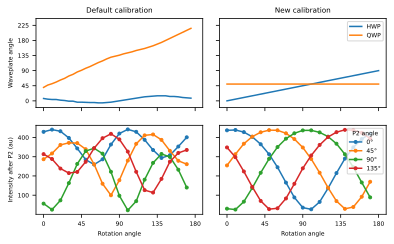
\includegraphics{detection_waveplate_calibrations.pdf}
	\caption{
		\todo{caption}
	}
	\label{fig:detection waveplate calibrations}
\end{figure}


\begin{figure}
	\centering
	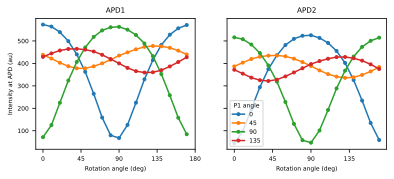
\includegraphics{pol_cube_effects.pdf}
	\caption{The POL cube distorts the polarisation state of incoming light. APD should measure the vertical component of the light (reflected by the POL cube), and APD2 should measure the horizontal component (transmitted). The detection waveplates were used to rotate incoming light, which was polarised along an angle shown in the legend. \todo{rephrase this! Its changing P1 that does it!!!}}
	\label{fig:pol cube effects}
\end{figure}


Second, I assessed both Abberior's and my calibration. As presented in \autoref{fig:detection waveplate calibrations}, my calibration works really well. \todo{Rephrase this entire paragraph! It is not entirely correct.} Finally, I also measured the polarisation characteristics of the POL cube. I generated linearly polarised light as in the previous paragraph, but left out P2. Then I rotated the polarisation using the detection waveplates and measured the intensity of light reflected and transmitted by the POL cube into APD1 and APD2 respectively. Apparently, the degree to which the POL cube can split the signal is strongly dependent on the polarisation of the light at the sample (the angle of P1), \autoref{fig:pol cube effects}. The cause of this effect is not immediately obvious, but is most likely due to some birefringence present in the POL cube.

\section{Conventional polarisation microscopy: acquisition and analysis}
\label{sec:pol analysis}
 
Because the current setup offers so much control over the light polarisation on both the excitation and detection ends, one can perform polarisation microscopy in several different ways:
\begin{enumerate}
	\item Measuring the intensity of emission components parallel and orthogonal to linearly polarised excitation ($ I_\parallel $ and $ I_\perp $). This is a very established method of polarisation microscopy, and allows for making anisotropy images, where every pixel is calculated according to
	\begin{equation}
		r=\frac{I_\parallel - I_\perp}{I_\parallel + 2I_\perp}.
	\end{equation}
	
	\item Detection of emission polarised at different angles after circular polarisation.
	
	\item Detection of total emission intensity as a function of the polarisation angle of excitation light.
\end{enumerate}

Methods 1 and 2 require the PBS cube to be placed in one of the FC housings. When placed in FC1, the PBS cube reflects $ s $-polarised light (horizontal) into APD1 and transmits $ p $-polarised light (vertical) to be collected by APD2. Unfortunately, we cannot use these methods yet, since they rely on the action of the detection waveplates, even if they are not actively rotating during the acquisition. Once we do, however, the waveplates can be used to sample more than two angles during an acquisition. This is necessary to distinguish between light polarised along \ang{+-45}, since these two angles give exactly the same intensity when sampling at \ang{0} and \ang{90} degrees.

The last method, however, is not subject to those constraints, and is already achievable on the Tegenfeldt microscope. I have carried out some acquisitions and wrote some code for analysing this data. The process of acquiring and analysing these images goes as follows:
\begin{enumerate}
	\item Acquire a stack of images at different excitation polarisation, for example at $ \theta_i = \ang{0}, \ang{10}, ..., \ang{170}$. Then we have a three-dimensional array of intensity values $ I_{ixy} $.
	\item Align images in this stack with each other, as the excitation beam seems to move as a function of polarisation angle. The alignment algorithm will be explained later.
	\item Compensate photobleaching
	\item For every pixel, calculate the Fourier coefficient corresponding to a period of \ang{180}.
	\item Based on that calculation, construct a new image in the HSV (hue, saturation, value) colour space where pixel colour depends on the polarisation direction, the saturation shows the degree of polarisation and the brightness (value) shows the total intensity of a pixel. 

\end{enumerate}

\paragraph{Stack alignment.} Images in a stack are aligned using an ECC optimisation algorithm partly implemented in the OpenCV software library \cite{Evangelidis2008}. The goal is to generate a new stack $ I'_{ixy} $ in which the drift is corrected. We will take the first frame as reference, setting 
\begin{equation}
	I'_{0xy} = I_{0xy}.
\end{equation}
For every other frame $ I_{ixy} $, we can calculate a warp matrix using the \texttt{findTransformECC()} method defined in OpenCV that maximises the correlation between $ I_{ixy} $ and $ I'_{(i-1)xy} $. We only calculate translational motion, so scaling and rotation are not allowed. Finally, we transform the original image using that warp matrix and \texttt{warpAffine()} and save the result as $ I'_{ixy} $, in other words:
\begin{equation}
	I'_{ixy} = \texttt{warpAffine}\left(
		I_{ixy}, 
		\texttt{findTransformECC}\left(I'_{(i-1)xy}, I_{ixy}\right)
	\right) \qq{for all} i>0.
\end{equation}

\paragraph{Bleaching compensation.} Since we want to calculate Fourier coefficient, we need to separate the photobleaching response from the polarisation response. We can do this by comparing two frames at identical polarisations and estimate the bleaching rate by their difference. Unfortunately, the Imspector software suite does not allow for rotating the excitation polarisation by more than \ang{175}, so we cannot do this exactly. We would be able to if we also used a PBS, but that is not an option, as explained before. For now, we simply estimate the bleaching rate based on the total intensity of the first and last frames $ I_0 $ and $ I_1 $ to be
\begin{equation}
	r = \left( \frac{I_1}{I_0} \right)^\frac{1}{n},
\end{equation}
given $ n $ number of frames were acquired. Then we can compensate for photobleaching by multiplying every frame with a correction factor as
\begin{equation}
	I'_{ixy} = r^{-i} I_{ixy}.
\end{equation}

\todo{Improve notation: $ I_1 $ for the last frame is confusing}

\paragraph{Colouring the image.} For every pixel, calculate a complex-valued Fourier coefficient corresponding to a period of \ang{180} (at which we should see polarisation dependence) using
\begin{align}
	F_{xy} &= \sum_i I_{ixy} e^{j2\theta_i},
\end{align}
where $ j $ is the imaginary unit. Then construct an image in the HSV (hue - orientation, saturation - degree of polarisation, value - total intensity) where 
\begin{align}
	h_{xy} &= \arg (F_{xy}),\\
	s_{xy} &= \abs{F_{xy}}/v_{xy},\\
	v_{xy} &= \sum_i I_{ixy}.
\end{align}
Finally, normalise these channels $ c $ to be in the range $ (0,1) $ and optionally apply a power law with a manually chosen coefficient $ \alpha_c $ for optimal visualisation,
\begin{equation}
	c'_{xy} = \left( \frac{c_{xy}}{\max (c_{xy})} \right)^{\alpha_c}.
\end{equation}
The effect of $ \alpha_c $ is presented in \autoref{sec:conventional pol}. \todo{todo}

\section{Polarisation-resolved STED microscopy (pSTED)}
\label{sec:methods psted}

Since polarisation is important to both excitation and emission of a fluorophore, it stands to reason that stimulated emission should also be polarisation dependent. In fact, that is what the calculation in Dyba et al.'s calculation of STED resolution is based on \cite{Harke2008, Dyba2005}. Moreover, excitation and stimulated emission are described by the same quantum mechanical process \cite{Foot}.

Would it then be possible to adapt the principle of conventional STED microscopy to increase the polarisation resolution of a microscope, instead of its spatial resolution? In this section, I will introduce a definition of polarisation resolution, a mathematical description of how this might be improved using pSTED, and how we adapted the microscope setup in order to achieve that. 

The general idea is that one can define a vectorial PSF (although a better term is photon fluence) that takes light polarisation into account. In a conventional polarisation microscopy setup, the probability of excitation of a fluorophore satisfies is proportional to $ \cos^2 \Delta\theta $, where $ \Delta\theta $ is the difference between the excitation polarisation and the transition dipole moment. This results in a FWHM resolution for conventional polarisation microscopy of 
\begin{equation}
	d_\theta = \ang{90}.
\end{equation}

\todo{This can also be seen from the fact that a cosine of any phase can be written as the sum of a cosine and a sine
\begin{equation}
	\cos(2\theta+\delta) = \cos\delta\cos 2\theta - \sin\delta\sin 2\theta.
\end{equation}
In other words: the sum of two cosines of a different phase }

By illuminating the sample with a depletion beam that is orthogonally polarised to the excitation laser, we can suppress fluorescence of fluorophores on the edge of this PSF, just like in conventional STED. This is illustrated in \autoref{fig:psted principle}.

\begin{figure}
	\centering
	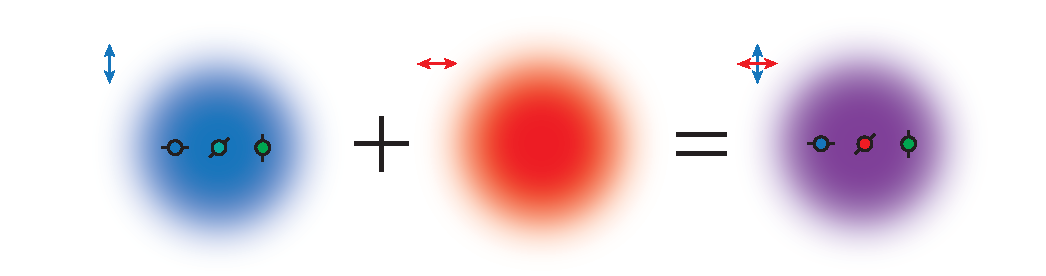
\includegraphics[width=\linewidth]{psted.ai}
	\caption{
		Illustration of the working principle of pSTED. The arrows outside indicate the polarisation of the laser light. The circles represent fluorophores with their transition dipole moment indicated by a line. The orthogonal polarisation of the depletion beam suppresses fluorescence of the fluorophore oriented at \ang{45}.
	}
	\label{fig:psted principle}
\end{figure}

\paragraph{Derivation of the pSTED PSF.} What follows is strongly inspired by Dyba et al.~\cite{Dyba2005}. Let $ \vb{x} = (x, y, z)$ be the spatial coordinates, $ \theta $ be an angle with the $ x $-axis in the $ xy $ plane (ranging from $ 0 $ to $ 2\pi$) and $ \phi $ be an angle with the $ z $-axis in the $ xz $ plane (ranging from $ -\pi $ to $+\pi$). \question{Delete mentions of $ z $ and $ \phi $?}

Let the fluorophore population be described by the density $ \rho(\vb{x}, \theta, \phi) $. This function is normalised such that its integral is equal to the number of fluorophores. For example, a single fluorophore at the origin, pointing in the $ x $ direction with no out-of-plane tilt would be described by the Kronecker delta distribution $ \rho_0 = \delta(\vb{x}, \theta, \phi) $.

The excitation beam is described by the electric field amplitude $ \vb{E}_\exc $, polarised along $ \theta_\exc $, and analogous for the depletion beam. Like \autoref{eq:convolution}, the emission intensity measured when the laser is focused on $ \vb{x}_\exc $ and polarised along $ \theta_\exc $ is now some sort of a convolution integral, where we have to integrate over both $ \vb{x} $ and $ \theta $ like
\begin{equation}
	I_\emm \propto \iint 
		\sigma_\exc \abs{\unit{n}_\theta\cdot \vb{E}_\exc(\vb{x}_\exc-\vb{x})}^2 
		\rho(\vb{x}, \theta) 
		\dd{\theta}\dd{\vb{x}} ,
\end{equation}
where $ \unit{n}_\theta $ is a unit vector pointing in the direction of $ \theta $. For the distribution $ \rho_0 $ and a constant intensity profile $ I_\exc = E_\exc^2 $, this reduces to
\begin{equation}
	I_\emm \propto \sigma_\exc I_\exc \cos^2\theta_\exc ,
\end{equation}
which is maximal when the excitation polarisation is in the $ y $ direction, as expected.

Now, we need to include the effect of the depletion field, which amounts to adding an exponential factor under the integral
\begin{equation}
	I_\emm \propto \iint
		\sigma_\exc \abs{\unit{n}_\theta\cdot \vb{E}_\exc(\vb{x}_\exc-\vb{x})}^2 
		\exp(-\sigma_\dep \abs{\unit{n}_\theta\cdot \vb{E}_\dep(\vb{x}_\exc-\vb{x})}^2)
		\rho(\vb{x}, \theta) 
		\dd{\theta}\dd{\vb{x}}.
	\label{eq:psted integral}
\end{equation}

If the two beams are orthogonally polarised, then $ \theta_\dep = \theta_\exc + \pi/2 $ and we can recover the following expression for the distribution $ \rho_0 $:
\begin{equation}
	I_\emm \propto 
		\sigma_\exc I_\exc \cos^2 \theta_\exc\cdot
		\exp(-\sigma_\dep I_\dep \sin^2 \theta_\exc)
	\label{eq:pol psf}
\end{equation}

This model can easily be extended to account for depolarising effects such as rotational diffusion, energy transfer, et cetera. However, that is not necessary at this point. Instead, we would like to know the resolution improvement this gives us. Unfortunately, I have not been able to solve for the FWHM resolution of the pSTED PSF, but I did calculate it numerically. Both an illustration of the PSF and the FWHM are presented in \autoref{fig:pol psf width}.

\begin{figure}
	\centering
	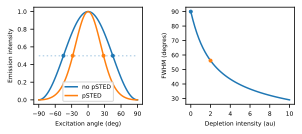
\includegraphics{pol_psf_width.pdf}
	\caption{\textbf{Left:} Narrowing of the fluorophore response as a result of a depletion field (of intensity $ I_\dep=2 $, as compared to the right pane). \text{Right:} Numerical calculation of the FWHM angular resolution $ d_\theta $ as a function of depletion intensity, based on \autoref{eq:pol psf}.}
	\label{fig:pol psf width}
\end{figure}

\paragraph{Implementation of pSTED.} The system was not set up for tuning the depletion polarisation. Instead, the STED polarisation is always circular, and this is ensured by a set of two fixed waveplates: a QWP and a HWP (refer to \autoref{fig:layout} and the description of the STED module in that section). 

To control the polarisation of the depletion beam, I first had to linearise the polarisation by compensating for the QWP in the beam path. That can be done by placing a QWP in the pSTED module in \autoref{fig:layout}. This works because 
\begin{equation}
	S_\qwp(\phi)S_\hwp(0)S_\qwp(-\phi) = R(2\phi).
\end{equation}
When the quarter-wave plates are aligned like that, this system simply rotates the polarisation by a fixed angle. Then, adding a HWP before this setup suffices to get full control over the polarisation angle of the depletion beam.

\section{Samples}
\label{sec:samples}

During the project, samples were very generously provided by research groups led by Pontus Nordenfelt and Vinay Swaminathan (Division of Infection Medicine, Faculty of Medicine, Lund University).

Results of the cell sample shown in the experimental section contain a human cell line infected with bacteria of the Yersinia genus. Stainings present are: DAPI (nucleus), GFP (bacteria) and SiR-actin. SiR-actin is an organic molecule (silicon-rhodamine) rigidly linked to an actin monomer. This dye is perfect for our setup, as SiR can be excited at 664~nm and has an sufficient absorption cross-section at 775~nm to perform STED. In addition, the fact that it is rigidly bound to the actin cytoskeleton means the light it emits is strongly polarised and reports on the the actin filament orientation.

I also used two control samples for calibration measurements. The first is a sample of small \question{How small?} reflective gold colloids, which were used to image the laser point spread functions. The second contains larger Tetraspec fluorescent beads (Invitrogen).